\documentclass[11pt]{article}
\usepackage[brazilian]{babel}
\usepackage[utf8x]{inputenc}
\usepackage[a4paper, total={6in, 8in}]{geometry}
\usepackage{enumitem}
\usepackage{pgfplots}
\usepackage{graphicx} 
\usepackage{float}
\pgfplotsset{width=10cm, compat=1.9}
\usepackage[framed,numbered,useliterate]{mcode}
\setlength{\parindent}{4em}

\begin{document}
% ========== Edit your name here
\author{
	José Fernando Rosa Ribeiro
}
\title{DAS5210 - Introdução ao Controle de Processos
	\newline
	\newline
	\large Prova 1
	\date{\vspace{-5ex}}}
\maketitle
\setcounter{secnumdepth}{0}

\section{Questão 1}
\begin{figure}[H]
	\centering
	{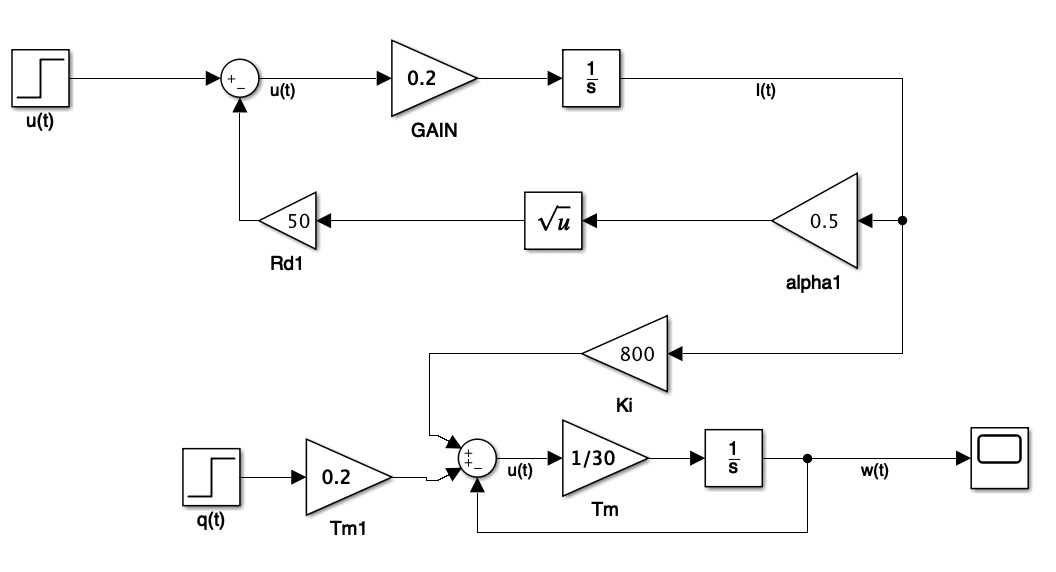
\includegraphics[width=\textwidth]
		{assets/q1_non_linearized_schema.jpg}}
	\caption{Diagrama do sistema não-linearizado no Simulink.}
\end{figure}

\begin{figure}[H]
	\centering
	{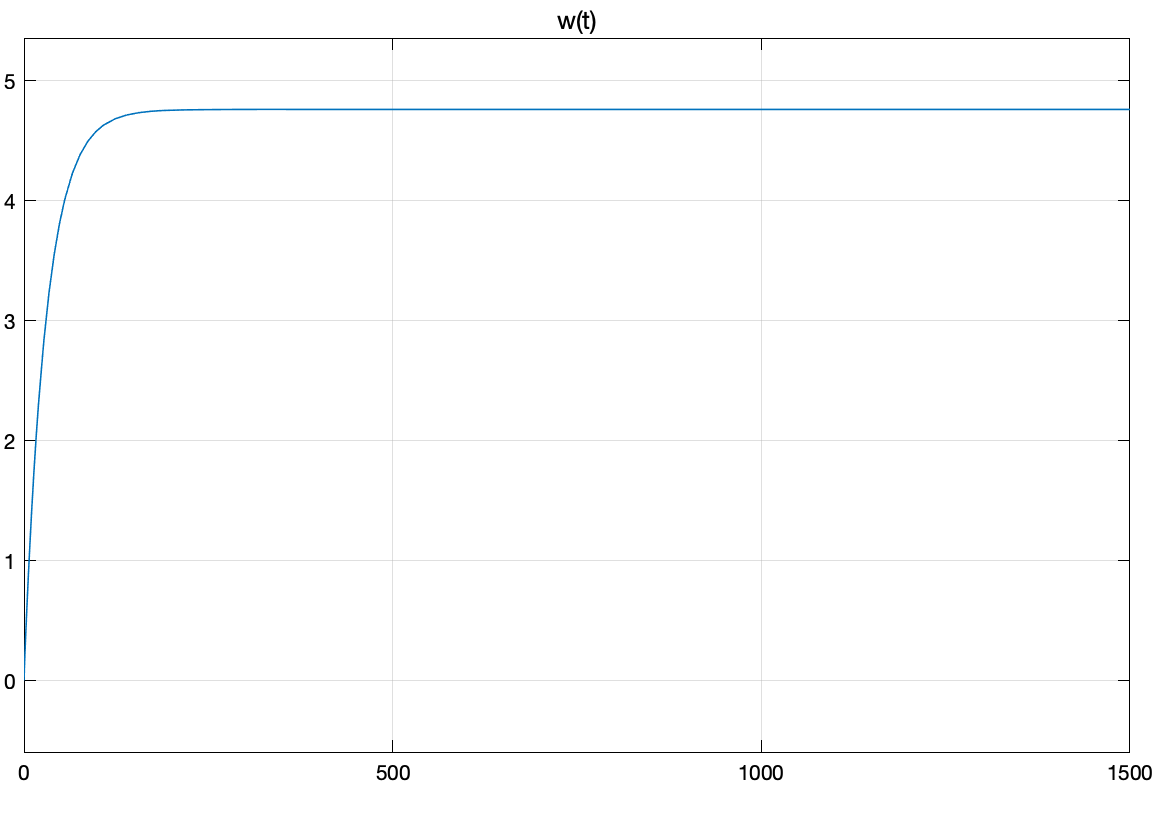
\includegraphics[width=\textwidth]
		{assets/q1_u(t)_3_q(t)_0to5.png}}
	\caption{Gráfico da variação de $\omega(t)$ com u(t)=5 e degrau q(t-1)=5}
\end{figure}

\begin{figure}[H]
	\centering
	{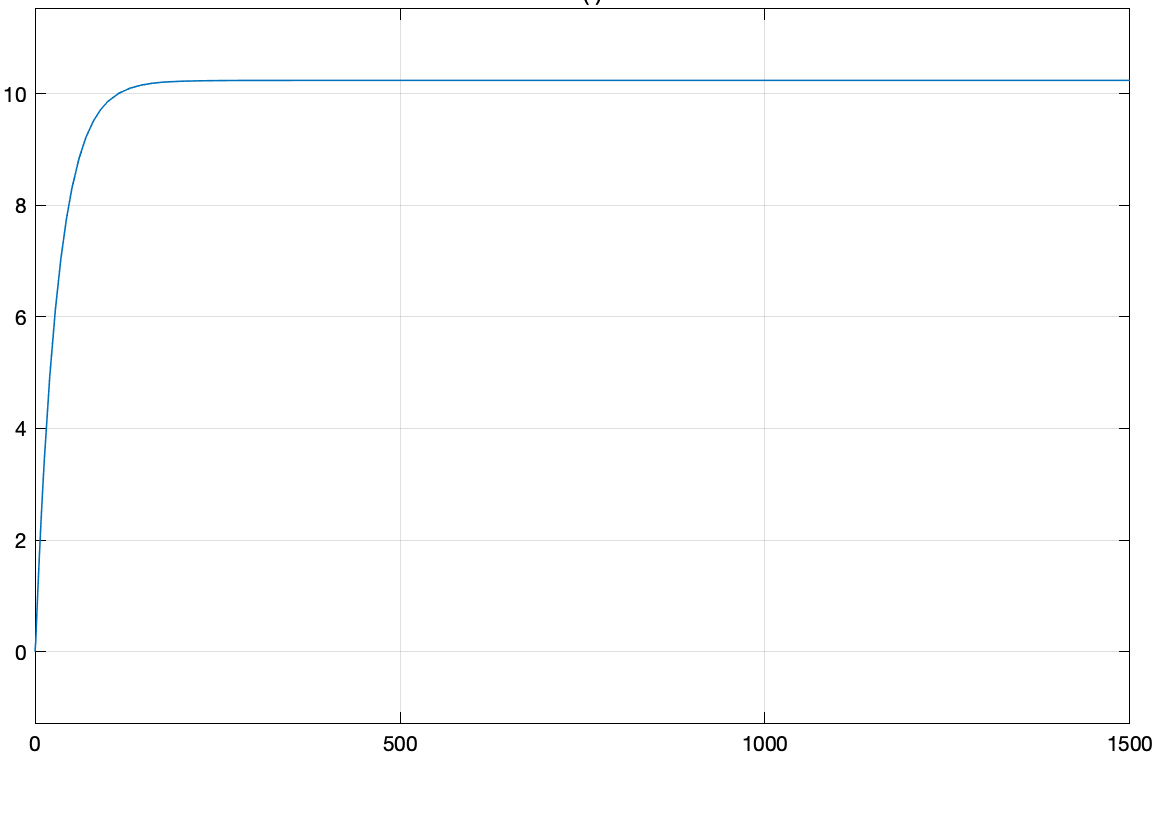
\includegraphics[width=\textwidth]
		{assets/q1_u(t)_3to4_q(t)_0.png}}
	\caption{ Gráfico da variação de $\omega(t)$ com degrau u(t-1)=3 a 4 e q(t)=0}
\end{figure}

\begin{figure}[H]
	\centering
	{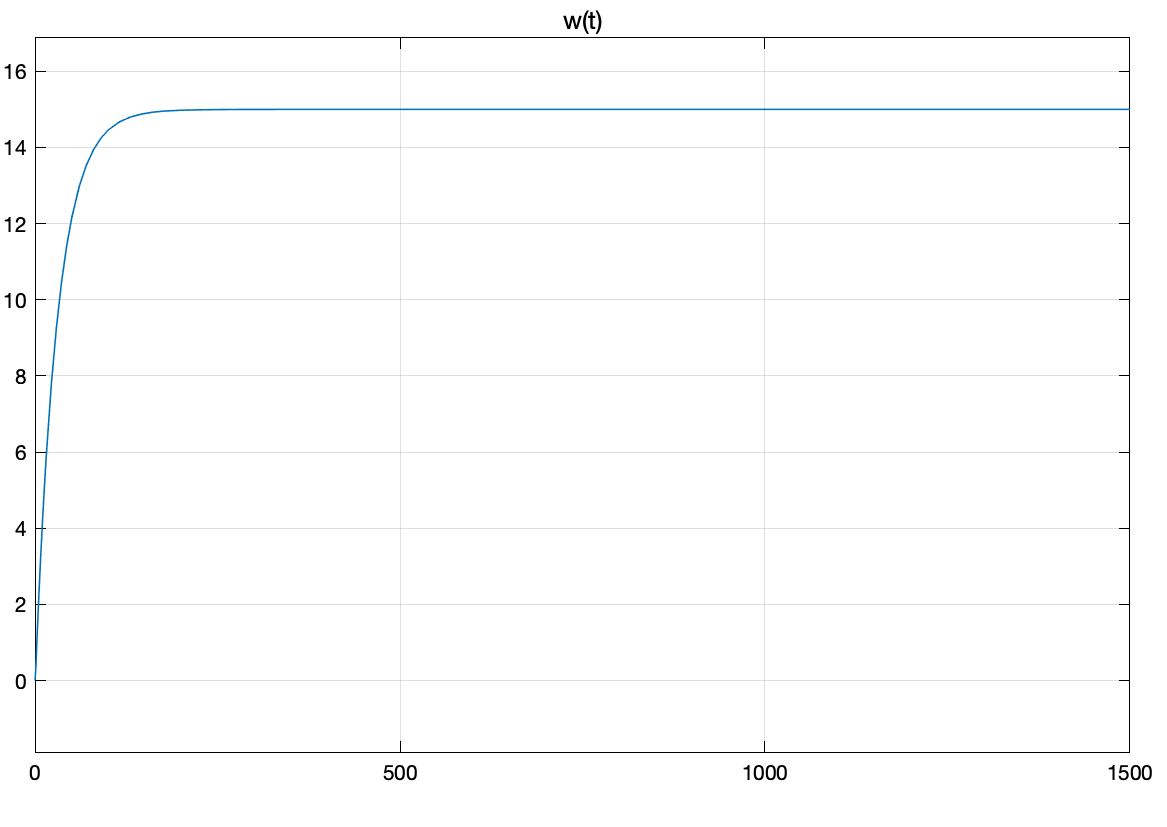
\includegraphics[width=\textwidth]
		{assets/q1_u(t)_4to5_q(t)_5.png}}
	\caption{ Gráfico da variação de $\omega(t)$ com u(t-1)=4 a 5 e q(t)=5}
\end{figure}

\section{Questão 2}

\begin{figure}[H]
	\centering
	{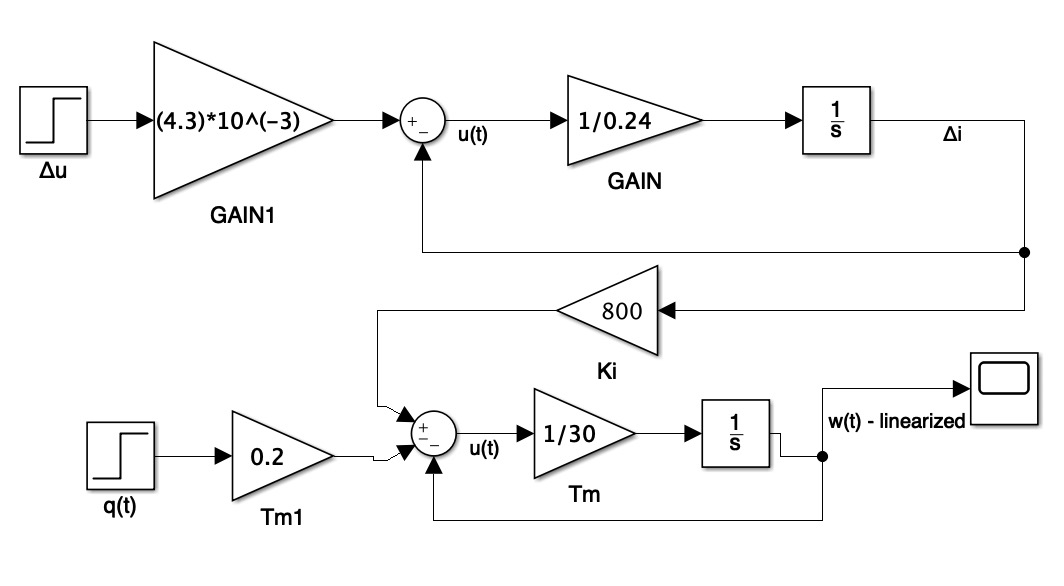
\includegraphics[width=\textwidth]
		{assets/q2_linearized_schema.jpg}}
	\caption{Diagrama do sistema linearizado.}
\end{figure}

\section{Questão 3}
Usando Simulink, estude por simulação o comportamento deste sistema e compare o comportamento
com o do sistema não-linear nas proximidades do ponto de equilibrio estudado. Use os mesmos ensaios
do item 1.

\section{Questão 4}
\subsection{Itens a e b}
\begin{lstlisting}[caption={Código usado para controlar a planta},captionpos=b]
function [y1, y2]= fcn(u, m)

lower_bound = 5;
upper_bound = 15;
active = m;
if active
    y1 = 5;
else
    y1 = 1;
end

if u>=upper_bound
    active = 0;
elseif u<=lower_bound
    active = 1;
end
y2 = active;
\end{lstlisting}

\begin{figure}[H]
	\centering
	{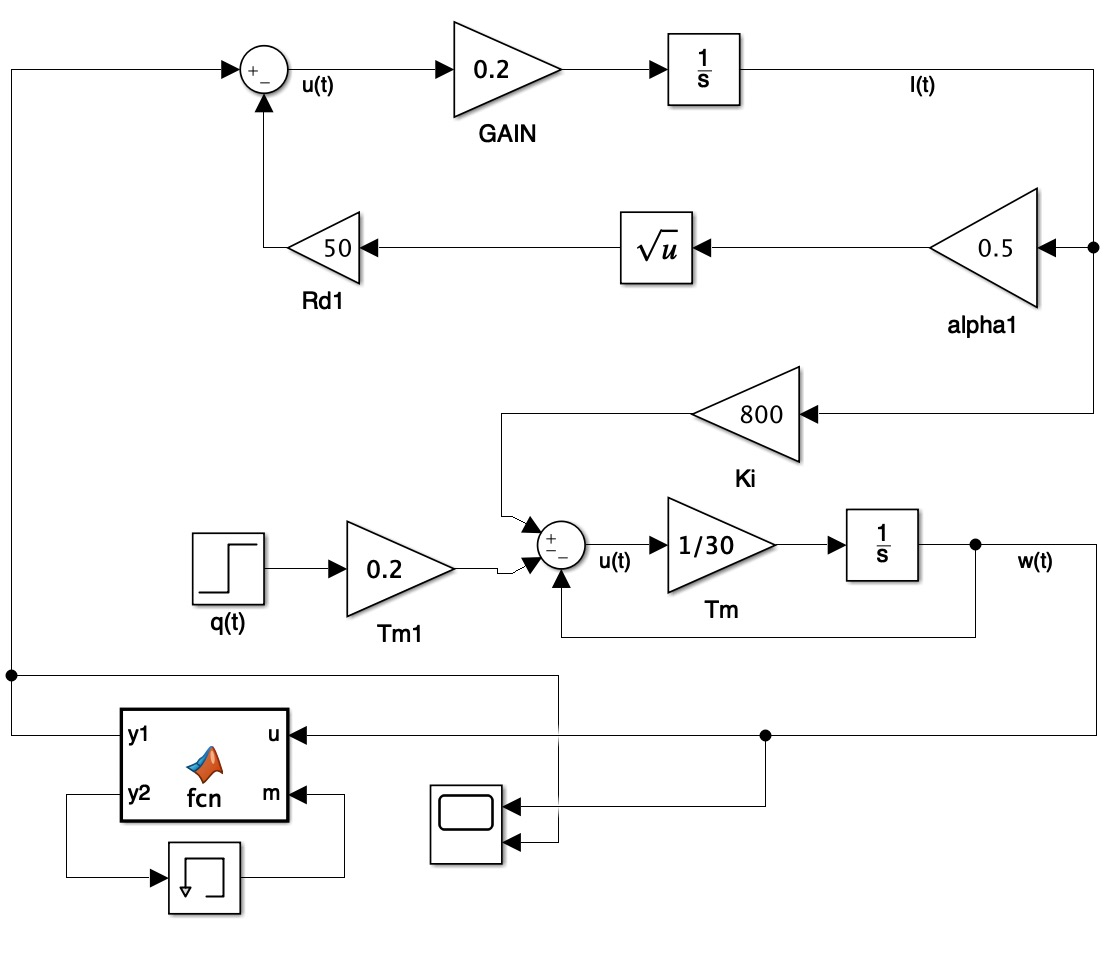
\includegraphics[width=\textwidth]
		{assets/q4_ab_control_schema.jpg}}
	\caption{Esquema da planta no Simulink.}
\end{figure}

\subsection{Item a}
\begin{figure}[H]
	\centering
	{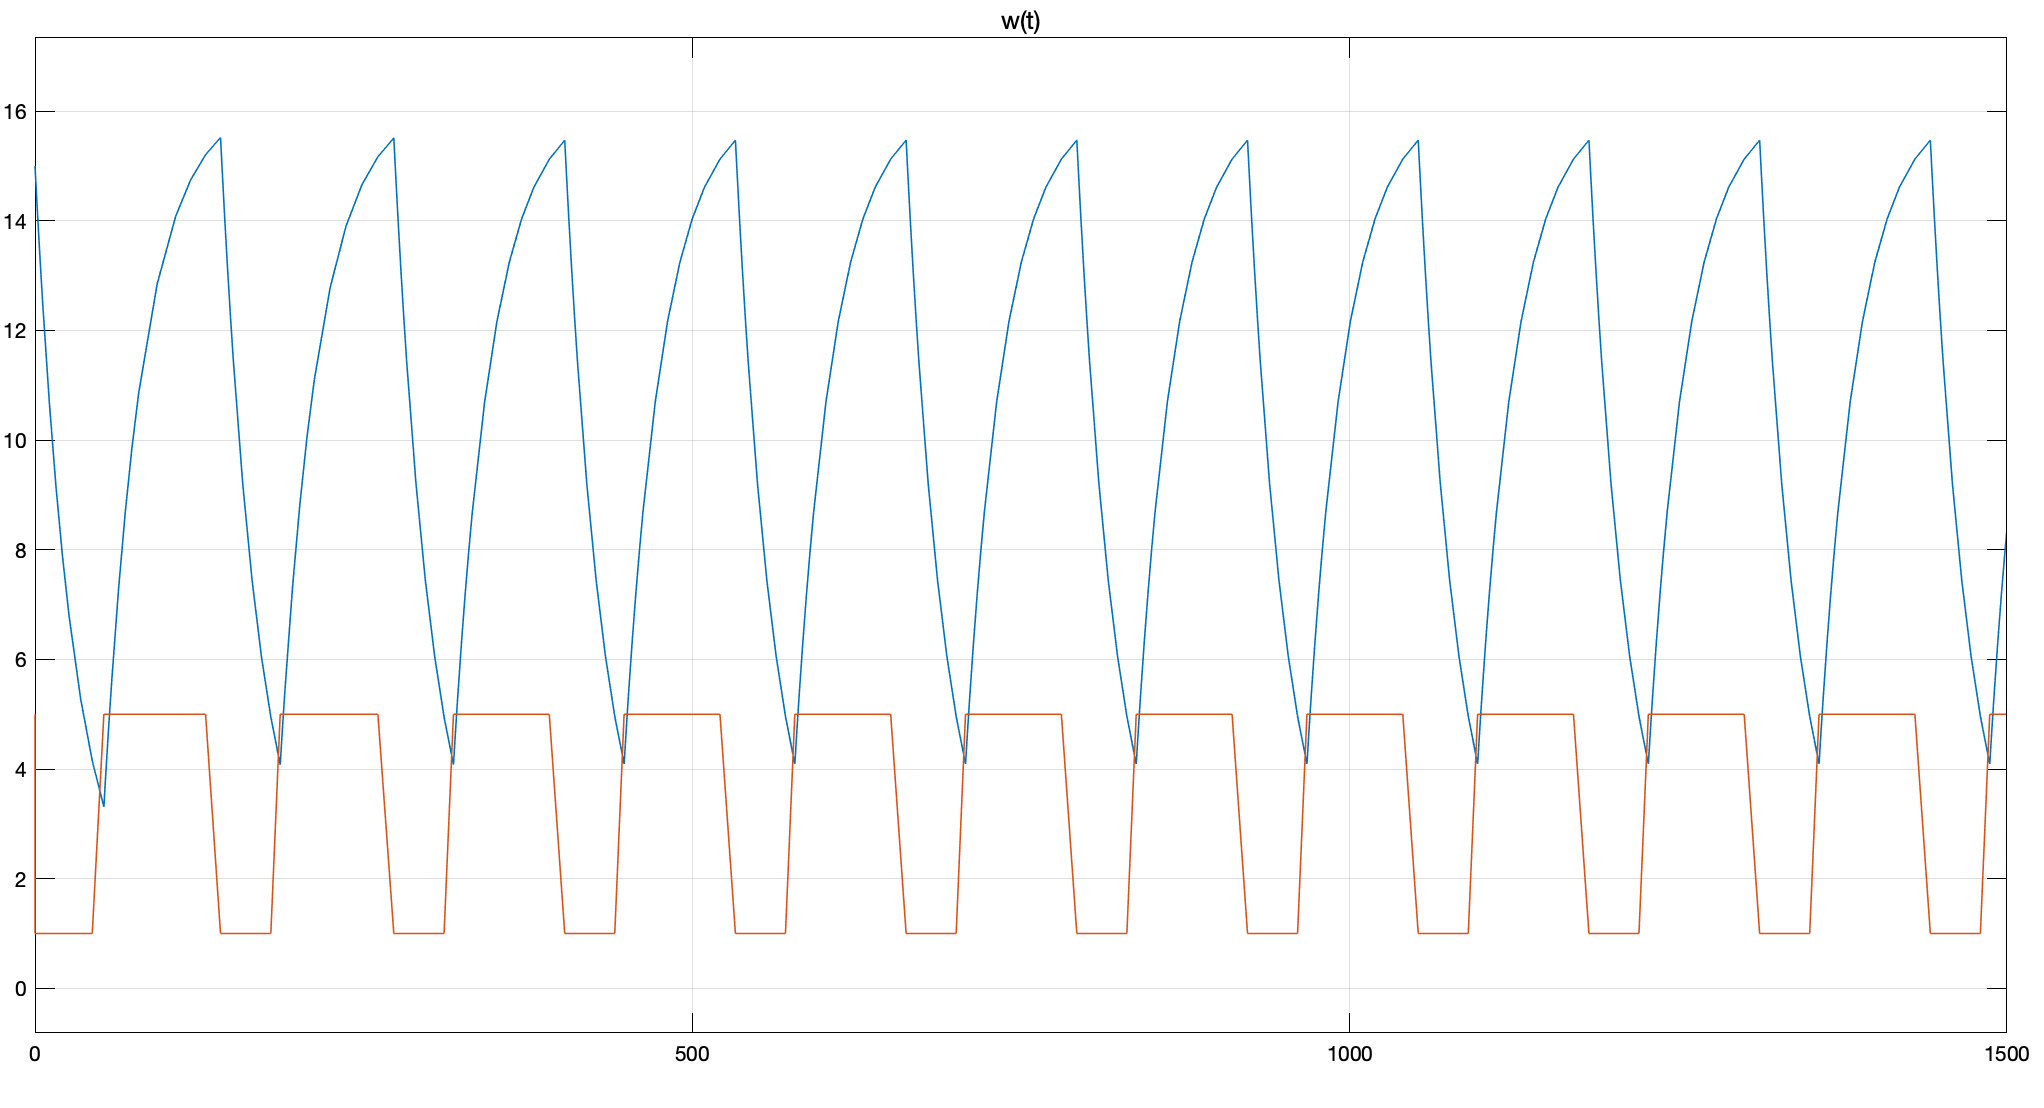
\includegraphics[width=\textwidth]
		{assets/q4_a_plot.png}}
	\caption{Gráfico de u(t) (em vermelho) e $\omega(t)$ (em azul), variáveis manipulada e controlada da planta, respectivamente, para $Q(t) = 1 N.m$}
\end{figure}

\subsection{Item b}
\begin{figure}[H]
	\centering
	{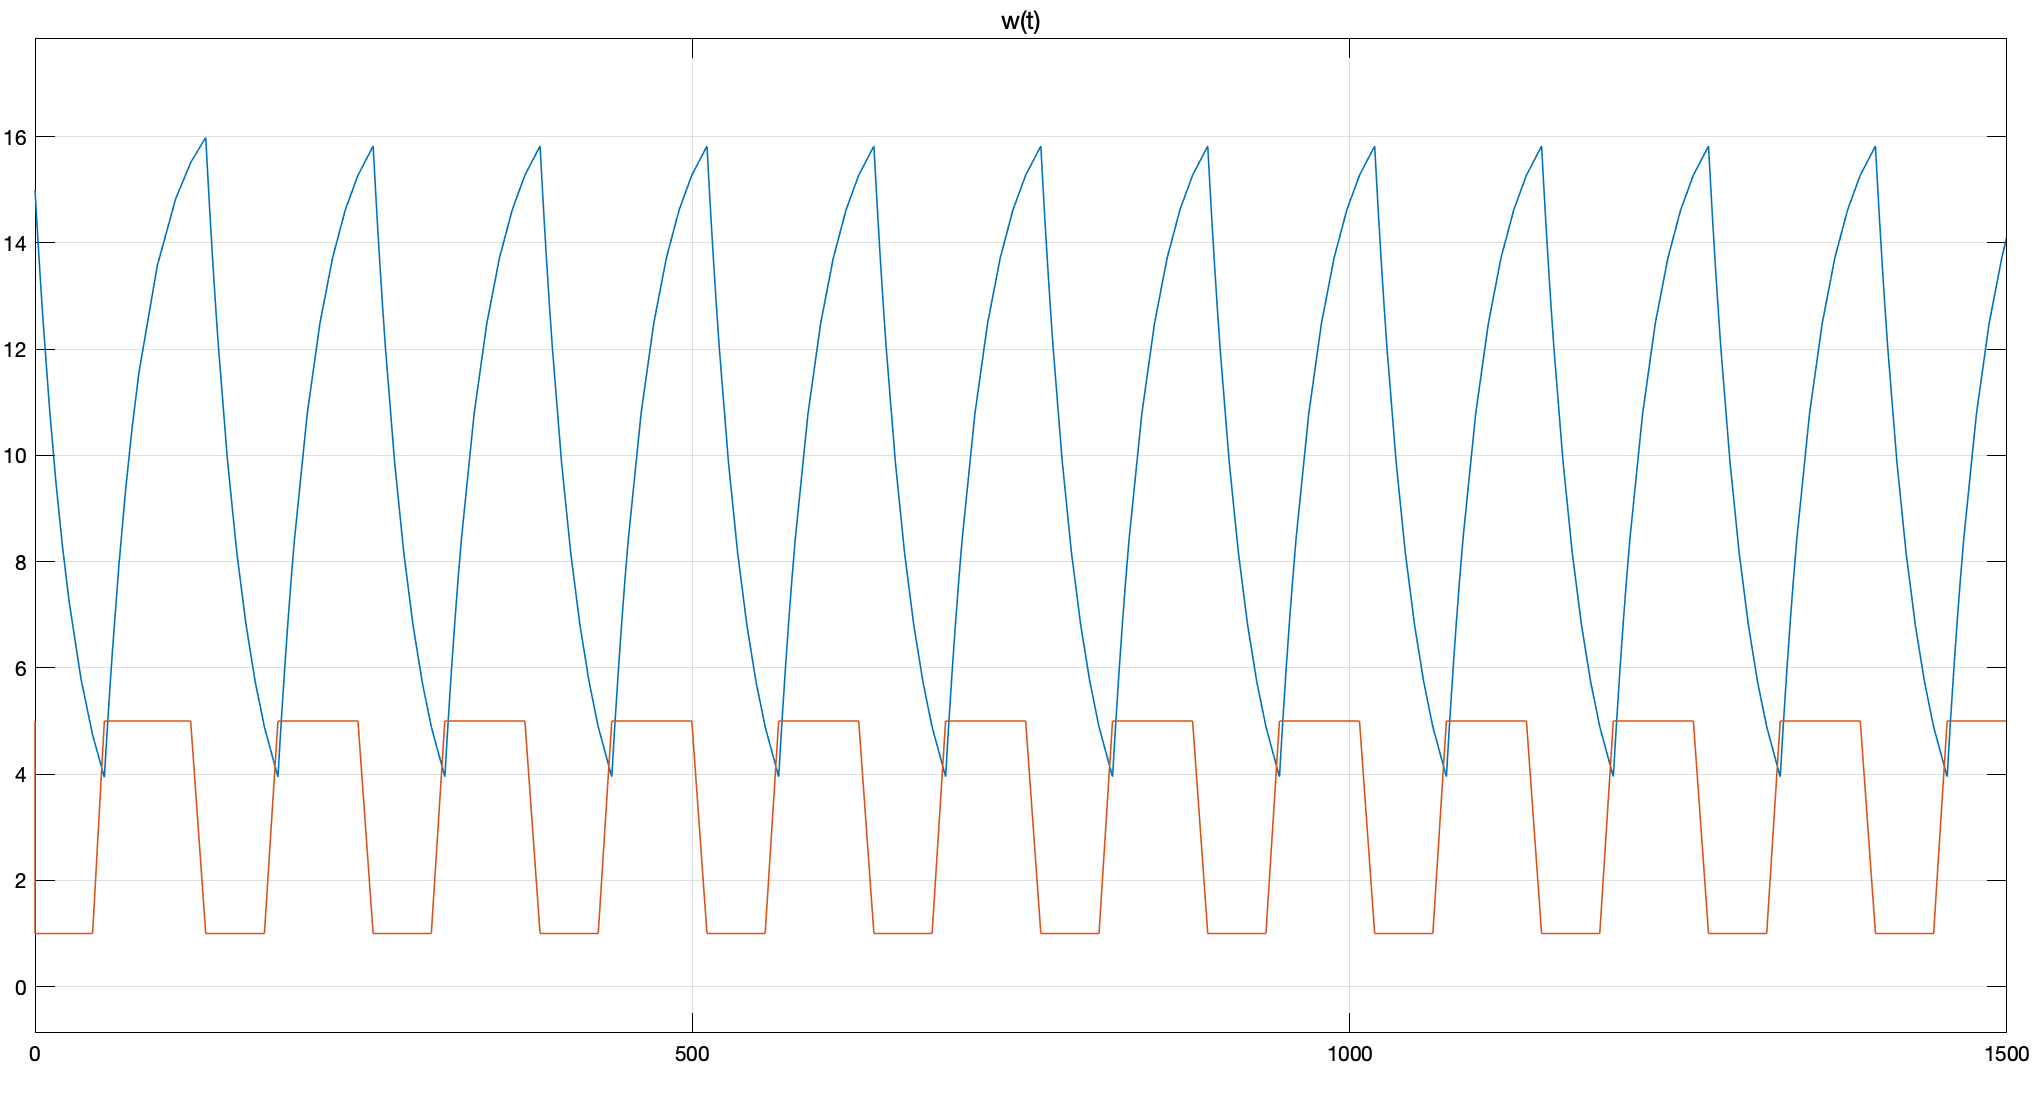
\includegraphics[width=\textwidth]
		{assets/q4_b_plot.png}}
	\caption{Gráfico de u(t) (em vermelho) e $\omega(t)$ (em azul), variáveis manipulada e controlada da planta, respectivamente, para $Q(t) = 5 N.m$}
\end{figure}

\subsection{Item c}

\begin{figure}[H]
	\centering
	{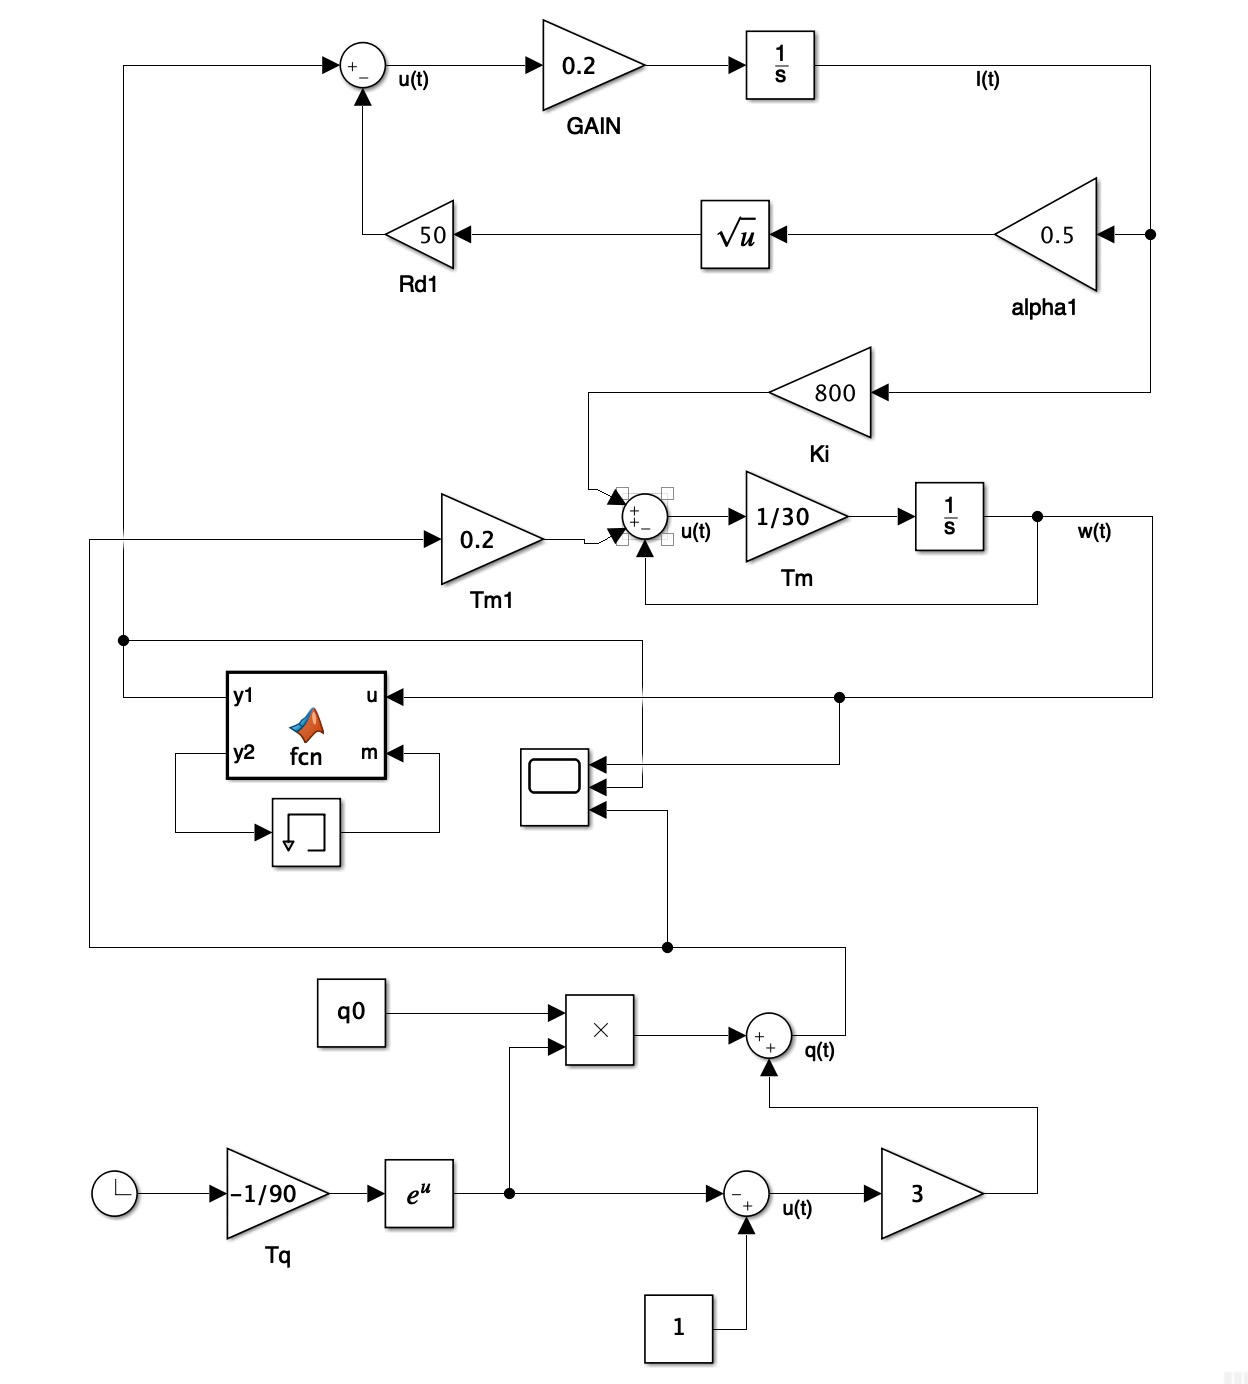
\includegraphics[width=\textwidth]
		{assets/q4_c_control_schema.jpg}}
	\caption{Gráfico de u(t) (em vermelho) e $\omega(t)$ (em azul), variáveis manipulada e controlada da planta, respectivamente, para $Q(t) = 5 N.m$}
\end{figure}

\begin{figure}[H]
	\centering
	{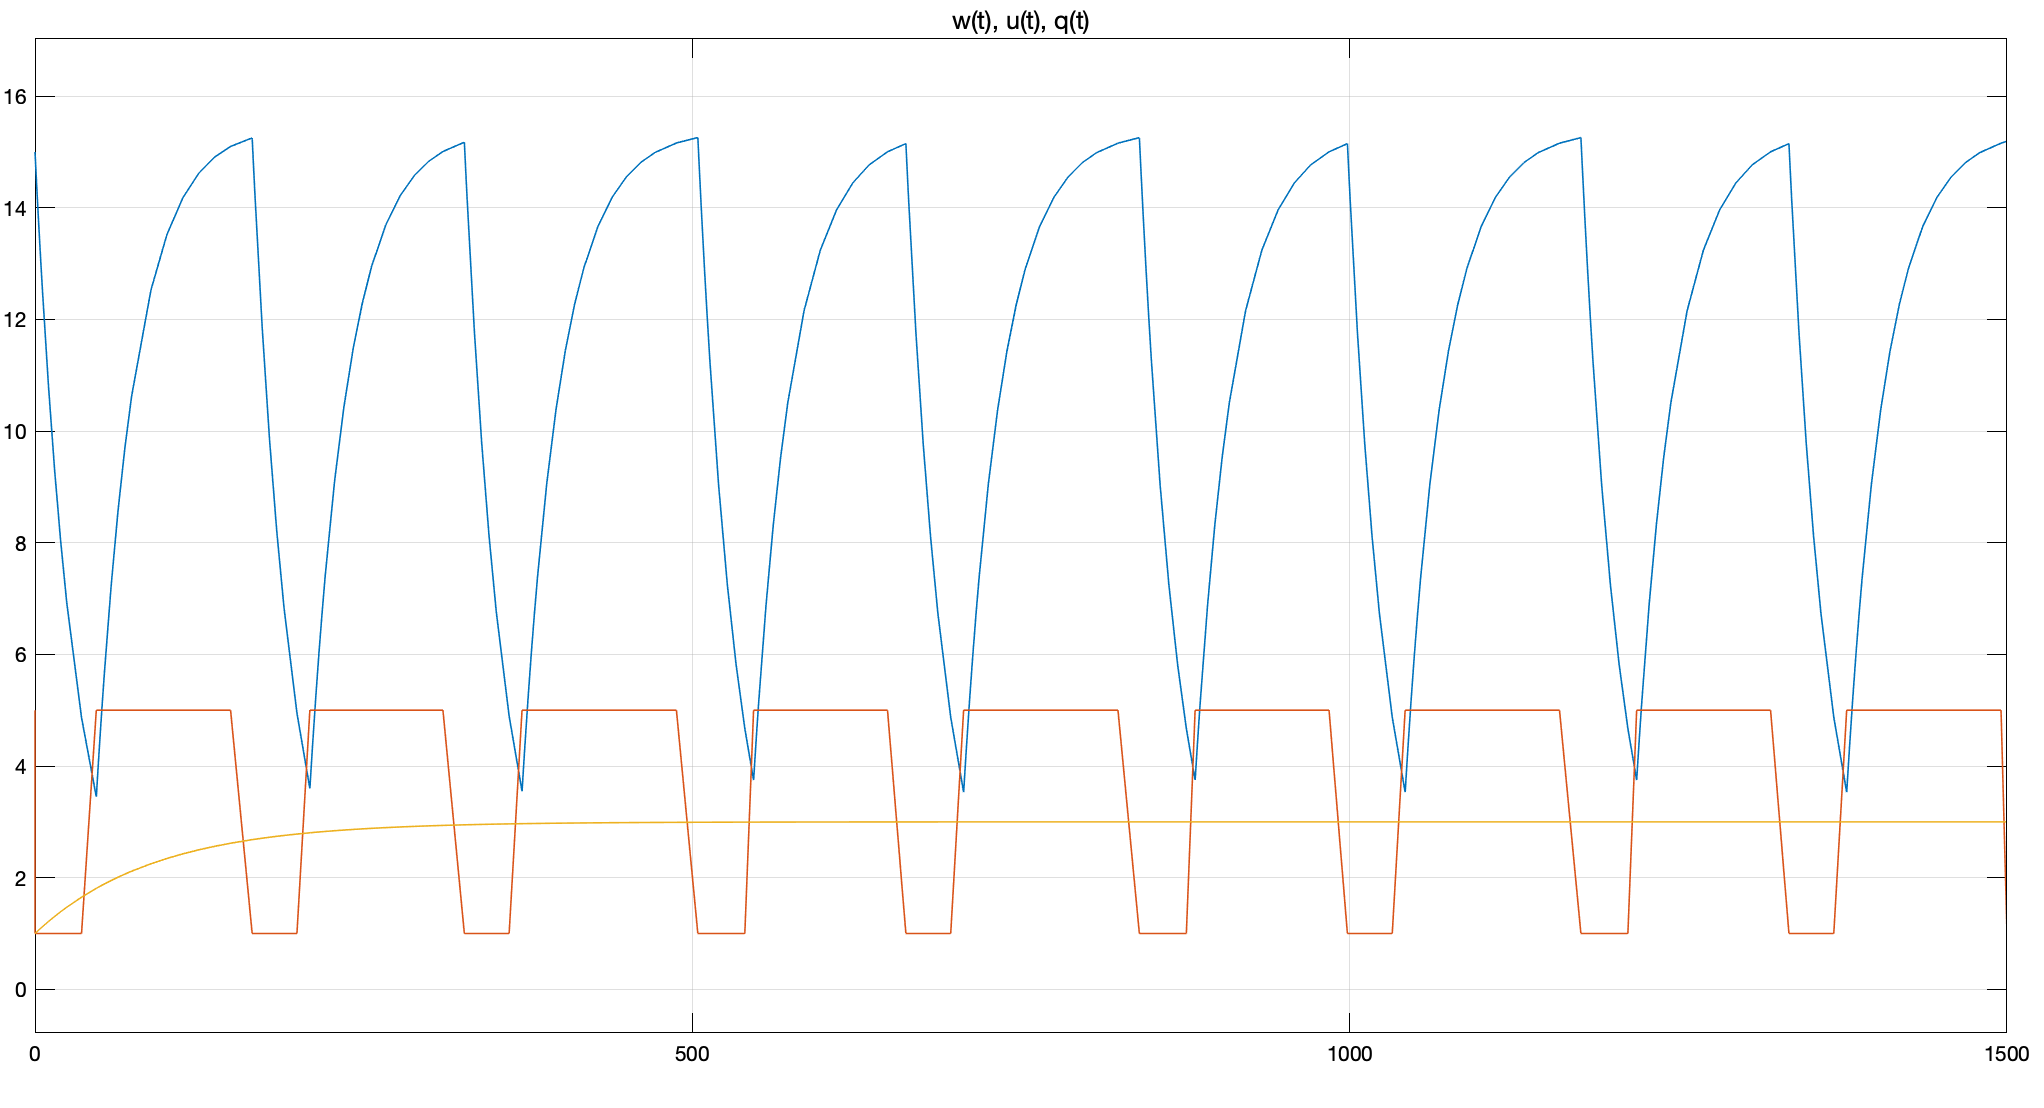
\includegraphics[width=\textwidth]
		{assets/q4_c_plot.png}}
	\caption{Gráfico de u(t) (em vermelho) e $\omega(t)$ (em azul), variáveis manipulada e controlada da planta, respectivamente, para $Q(t) = 5 N.m$}
\end{figure}


\section{Questão 5}
Pretende-se "controlar” o sistema de velocidade do motor em malha-aberta, usando uma lei de
controle do tipo u(t) = KMAr(t), sendo r(t) uma referência de velocidade do tipo degrau. Ajuste o
ganho KMA e analise separamente as respostas temporais i(t) (considere variações do tipo degrau). É
possível, com esta estratégia, garantir o seguimento de referências de velocidade r(t) do tipo degrau
?
\section{Questão 6}
Compare a estratégia de controle acima com a estratégia On-Off e avalia as capacidades de ambas
em termos de seguimento de referência e rejeição de perturbações q(t) do tipo degrau.
\end{document}
